\documentclass[cheatsheet.tex]{subfiles}
\begin{document}
means learning (typically binary) concepts from examples. The learned concept is the positive class. Everything else is the negative class. In concept learning, we want to learn a Boolean function over a set of attributes+values. The target concept c is the true concept. The \textbf{hypothesis} is a Boolean function over the features.
\\
\textbf{challenge} decide which hypothesis is best, given the training data, we want to learn a concept that will generalize well to new, unseen instances.
\subsection{hypothesis space}
The space of all possible concepts is called the hypothesis space. how many possible instances are there for a given set of features: $F_1 \times F_2 \times F_N$. All combinations of feature values. The hypothesis space is the number of binary functions on these instances $2^{F_1 \times F_2 \times F_N}$. 
\\
\textbf{conjunctive hypothesis space} hypotheses that can be expressed as a conjunction of literals. add not care to each feature. (F1+1)x(F2+1)x(FN+1). In this conjunctive hypothesis space, we can't represent concepts like "all courses in AI or Graphics". 
\\
\textbf{CHS learning} a specific-to-general approach in coming up with a hypothesis. 
\subsection{pathes through hypothesis space}
Every node connects upward to every more general hypothesis that includes it. Number of Donot know increases by 1 each level. Note that \textbf{True} can be appended to any proposition, so this is what's left when all the literals are removed.
\\
\textbf{Reducing the hypothesis space} rule out all the hypotheses (concepts, nodes) that don't include at least one of the instances in our example. choose the least general. 
\\
\textbf{Least general generalization (LGG)} We want to generalize beyond our specific training data, but not too much -- the most general hypothesis is to accept everything.  the more general our hypothesis, the lower our False negative rate. less general our hypothesis, the lower our False positive rate. \\
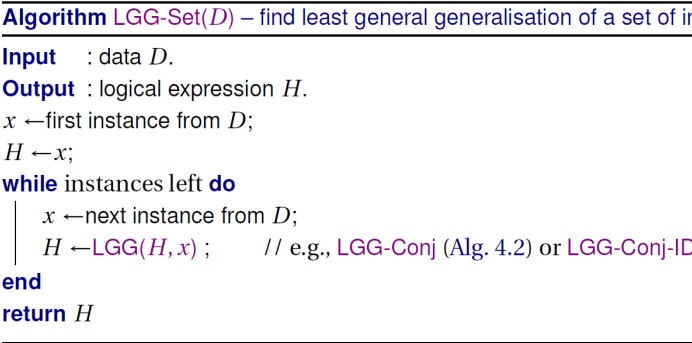
\includegraphics[width=0.8\linewidth]{LGG-set.png}
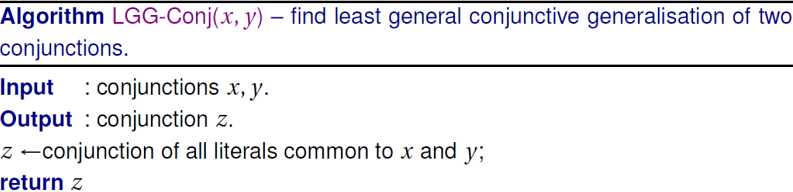
\includegraphics[width=0.8\linewidth]{LGG-Conj.png}\\
\textbf{Negative examples} help to prune the hypothesis space. Rule out hypotheses that include negative examples. 
\\
\textbf{internal disjunction} $(2^{F1}-1)(2^{F2}-1)(2^{Fn}-1)$ When all values of a feature are included, the feature becomes donot care. 
\\
\textbf{Additional note} \textbullet The number of hypotheses consistent with the data: For a given training data example, which is a leaf node at the lowest level in the graph, all connected nodes above it (including the data point itself) are hypotheses consistent with that data point. Adding a new, different data point prunes the nodes that represent hypotheses consistent with both data points. \textbullet The generality of various hypotheses: Higher/lower nodes represent more/less general hypotheses.
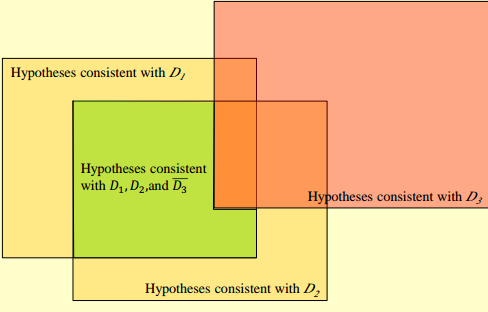
\includegraphics[width=.8\linewidth]{venn.png}
\\
\textbf{Algorithm} (starting with the first data point as the initial hypothesis and generalizing with more data points) prunes hypotheses at each step, choosing the least general consistent hypothesis as the current hypothesis. \textbf{Adding a positive/negative training example} prunes the space of consistent hypotheses by eliminating hypothesis that \textbf{do not/do} have a link to the new example. A negative example will always prune the top node (True)
\subsection{beyond conjunctive concepts}
skip
\subsection{learnability}
\textbf{Hypothesis languages} can be extended to more realistic data by modifying the "all or nothing" nature of positive/negative training data. We can make richer hypothesis representation languages: CHS, CHS with internal disjunctions, Conjunctions of Horn clauses, Clauses in first-order logic. The richer the representation and thus the more expressive the hypothesis language, the more difficult the learning problem. 
\\
\textbf{Complete and consistent} A concept is complete if it covers all positive examples. A concept is consistent if it covers none of the negative examples. The version space is the set of all
concepts that are both complete and consistent. 
\\
\textbf{PAC learning} Probably Approximately Correct. PAC outputs, with probability at least $1-\sigma$ (most of the time), a hypothesis h such that $err_D < \epsilon$ (mostly right). we can guarantee this by choosing a large enough training set $|D| \geq \frac{1}{\epsilon}(ln|H|+ln\frac{1}{\sigma})$ This leads to the concept of \textbf{VC dimension}. 

\end{document}





